\documentclass[11pt]{article}
\usepackage[utf8x]{inputenc}
\usepackage[english]{babel}
\usepackage{graphicx}
\usepackage{wrapfig}
\usepackage[margin=3cm, tmargin=2cm]{geometry}
\usepackage{color}
\usepackage{hyperref}
\usepackage{array}

\begin{document}
 \bibliographystyle{plain}%Choose a bibliograhpic style
\title{Network training}
\date{Fall 2014}
\author{Maël Auzias}
\maketitle

\tableofcontents
\pagebreak


\section{Introduction}
\subsection{Classification}
Give a concrete example of each of the following kinds of networks (name some devices):
  \begin{enumerate}
    \item BAN,
    \item PAN,
    \item LAN,
    \item WAN.
  \end{enumerate}

\subsection{Topologies}
Give a concrete example of each of the following network topologies:
  \begin{enumerate}
    \item Bus,
    \item Star,
    \item Fully connected.
  \end{enumerate}

\subsection{TCP connection}
According to TCP (\color{blue}\href{http://tools.ietf.org/html/rfc761}{RFC761 (January 1980)}) \color{black}, what are the sequences used in order to establish a connection between two hosts?

\subsection{TCP or UDP?}
\subsubsection{Sensors}
You are creating a network application using sensors. The sensors can receive requests to change their settings (rate of measurement, range...) and they continuously send their measurements.
  \begin{enumerate}
    \item Should request packets (settings) be sent with UDP or TCP? Why?
    \item Should measurement packets be sent with UDP or TCP? Why?
  \end{enumerate}
\subsubsection{Website}
Does HTTP (\color{blue}\href{http://tools.ietf.org/html/rfc2616}{RFC2616 (June 1999)}) \color{black} rely on TCP or UDP? Why?

\subsection{FTP}
\subsubsection{Is FTP secure?}
According to the file \color{blue}\href{http://teaching.auzias.net/db/ftp-connect.pcap}{ftp-connect.pcap} \color{black} is FTP secure? What could you do to use it more securely?
\subsubsection{FTP and TCP}
According to the file \color{blue}\href{http://teaching.auzias.net/db/ftp-disconnect.pcap}{ftp-disconnect.pcap} \color{black} does FTP respect the TCP protocol to close a connection?

\subsection{DNS}
\subsubsection{Some news}
According to the file \color{blue}\href{http://teaching.auzias.net/db/nslookup.pcap}{nslookup.pcap} \color{black} what is:
  \begin{enumerate}
    \item the DNS server?
    \item the domain name for which the IP address is needed?
    \item the IP address of the domain if any?
  \end{enumerate}n
\subsubsection{Which one?}
According to the file \color{blue}\href{http://teaching.auzias.net/db/nslookup-whoseone.com.pcap}{nslookup-whoseone.com.pcap} \color{black} what is:
  \begin{enumerate}
    \item the DNS server?
    \item the domain name for which the IP address is needed?
    \item the IP address of the domain if any?
  \end{enumerate}

\subsection{Ping-pong}
\subsubsection{Are you there?}
According to the file \color{blue}\href{http://teaching.auzias.net/db/ping.pcap}{ping.pcap} \color{black}:
  \begin{enumerate}
    \item what is the node 127.0.0.1 doing?
    \item Is the node 127.0.0.2 on the network?
  \end{enumerate}
\subsubsection{Who has this IP?}
According to the file \color{blue}\href{http://teaching.auzias.net/db/arp.pcap}{arp.pcap} \color{black} and to ARP (\color{blue}\href{http://tools.ietf.org/html/rfc826}{RFC826 (November 1982)})\color{black}. What is the source trying to do? What is ARP used for? If ever a host does not respond to ping (i.e., for security reasons), how could you check if the host is up anyway ?


%%%%%%%%%%%%%%%%%%%%%%%%
%%      Layer 1       %%
%%%%%%%%%%%%%%%%%%%%%%%%
\section{Physical layer}
\subsection{General}
\subsubsection{Aims}
What are the layer-1 goals?
\subsubsection{Name it}
What are the common (\emph{commercial}) name of:
  \begin{enumerate}
    \item IEEE 802.11
    \item IEEE 802.15.1
    \item IEEE 802.15.4
  \end{enumerate}
What is IEEE 802.15 related to? What does WPAN stand for?

\subsection{Encoding, encrypting, decoding}
It is important to know what are the differences between encoding and encryption. Following questions are related to theses subjects.
\subsubsection{Encrypt?}
What are the differences between encoding and encryption?\\
What are the two main kinds of encryption? Their advantages?\\
Name three well known cryptographic methods and three well known encoding methods.

\subsubsection{Encode it}
The string \verb$"Zp"$ (which does not mean anything but has a nice binary value!) is, according to ASCII, \verb$0x5a70$. Encode it using:
  \begin{enumerate}
    \item Multi-Level Transmit
    \item Alternate Mark Inversion
    \item Manchester (or differential Manchester)
    \item Biphase Mark Code
  \end{enumerate}

\subsubsection{Decode it}
What are the ASCII characters of theses images:
  \begin{figure}[h]
    \centering
    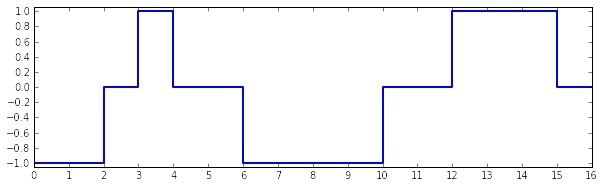
\includegraphics[height=3cm]{../slides/imgs/MLT3:).jpg}
    \caption{MLT3 encoded}
    \label{fig:mlt3}
  \end{figure}
  \begin{figure}[h]
    \centering
    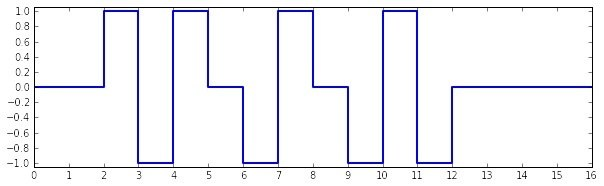
\includegraphics[height=3cm]{../slides/imgs/AMI;p.jpg}
    \caption{AMI encoded}
    \label{fig:ami}
  \end{figure}

\subsection{For\emph{Oh}For error}
\subsubsection{Calculate it}
What would be the output of the binary: \verb$0b0011 0000 1110 1001$ using the error detection methods:
  \begin{enumerate}
    \item Repetition (2)
    \item Parity (odd)
    \item Parity (even)
    \item Checksum (over 4 bit)
    \item MD5 hash
  \end{enumerate}

\subsubsection{Validate it}
Are theses received data correct? NB: detection values are in square brackets.
  \begin{enumerate}
    \item Using repetition (2), was received: \verb$0b0011 0011 0000 0000 1110 1001 1001 1001$
    \item Using parity (odd), was received: \verb$0b1011[1] 1010[0] 1100[1] 0111[1]$
    \item Using parity (even), was received: \verb$0b1011[1] 1010[0] 1100[1] 0111[1]$
    \item Using checksum (over 4 bit), was received: \verb$0b0011 0111 0010 0010 1110 1001 1101 1001 [1011]$
    \item Using MD5, was received the string (without the quotes!): \verb$"that's way too long..."$ the md5 sum: \verb$[3be37cad170213a8ad936c0640e3238b]$
  \end{enumerate}


\subsubsection{Correct it}
By using MDPC (Multidimensional parity-check code) the data received are: \verb$0x01 09 0e 06 03 09 0b 0c$. Are the data correct? What would be the correction? \\
  \begin{figure}[h]
    \centering
    \begin{tabular}{cc|c}
      0x01 & 0x09 & 0x0e \\
      0x06 & 0x03 & 0x09 \\ \hline
      0x0b & 0x0c &
    \end{tabular}
    \caption{Data received with MDPC}
    \label{fig:ami}
  \end{figure}

\end{document}
